\documentclass{fizykalab}

% Ustawienia do tabelki

\wydzial{WI}
\autorjeden{Dawid Komęza}
\autordwa{Magdalena Śmietana}
\rok{II}
\grupa{14}
\zespol{2}
\temat{Busola stycznych}
\nrcwiczenia{41}
\datawykonania{14.11.25}
\dataoddaniajeden{}
\zwrotdopoprawy{}
\dataoddaniadwa{}
\datazaliczenia{}

\begin{document}

\maketitle


\section{Cel ćwiczenia}
Celem ćwiczenia jest zapoznanie się z przyrządem zwanym \emph{busolą stycznych} oraz z metodą jego stosowania. Eksperymentalnie zostanie określona pozioma składowa ziemskiego pola magnetycznego $B_0$.

\section{Wstęp teoretyczny}
Zgodnie z prawem Biota–Savarta, dla pojedynczego zwoju cewki wartość wytworzonej przez prąd indukcji magnetycznej wyraża się wzorem:
\begin{equation}
d\vec{B} = \frac{\mu_0 I}{4 \pi} \frac{d\vec{l} \times \vec{r}}{|\vec{r}|^3}.
\end{equation}
Znaczenie poszczególnych symboli przedstawiono na rysunku ponizej.

Dla magnesu umieszczonego w środku cewki wektor $\vec{r}$ jest stały o długości $R$. Ponieważ wektory $d\vec{l}$ i $\vec{r}$ są prostopadłe, mamy:
\begin{equation}
d\vec{l} \times \vec{r} = |d\vec{l}| \cdot R.
\end{equation}

\begin{figure}[h!]
    \centering
    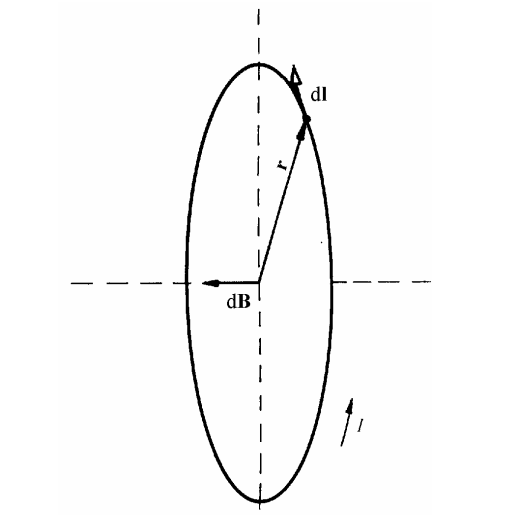
\includegraphics[width=0.4\textwidth]{cewka.png}
    \caption{Zastosowanie prawa Biota - Savarta do pojedynczego zwoju cewki.}
    \label{fig:cewka}
\end{figure}

Suma wektorów $d\vec{l}$ dla całego okręgu wynosi $2\pi R$. Dla cewki złożonej z $N$ zwojów ostateczna wartość pola magnetycznego w jej środku wyraża się wzorem:
\begin{equation}
B = \frac{\mu_0 N I}{2 R}.
\end{equation}

\section{Aparatura}
Do przeprowadzenia doświadczenia wykorzystano:
\begin{itemize}
    \item Amperomierz analogowy, służący do pomiaru natężenia prądu w obwodzie (klasa dokładności 0,5).
    \item Cewkę elektryczną o średnicy $d = 0,26 \pm 0,003$~m, z możliwością zmiany liczby zwojów, przez które przepływa prąd.
\end{itemize}

Dodatkowo użyto:
\begin{itemize}
    \item przełącznika do zmiany kierunku przepływu prądu,
    \item zasilacza pozwalającego regulować natężenie prądu,
    \item kątomierza z linijką do pomiaru wychylenia igły busoli.
\end{itemize}

Schemat połączeń przedstawiono na rysunku~\ref{fig:uklad}.

\begin{figure}[h!]
    \centering
    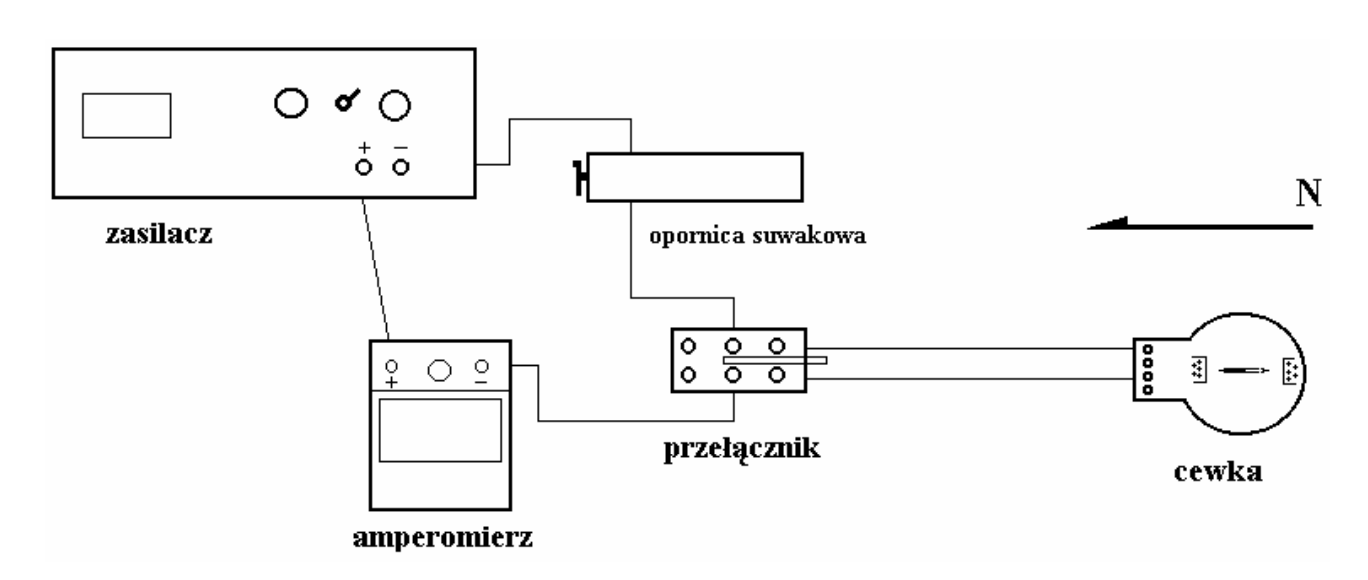
\includegraphics[width=0.6\textwidth]{uklad_busoli.png}
    \caption{Schemat układu elektrycznego busoli stycznych.}
    \label{fig:uklad}
\end{figure}

\section{Przebieg ćwiczenia}
Doświadczenie rozpoczęto od ustawienia amperomierza na zakres 0,75~A oraz podłączenia pozostałej aparatury. Następnie, dla różnych wartości natężenia prądu, mierzono wychylenie igły busoli za pomocą kątomierza, wykonując po sześć pomiarów dla danej liczby zwojów. Liczbę zwojów zmieniano czterokrotnie.

Wyniki pomiarów oraz obliczone wartości indukcji magnetycznej $B$ dla wzoru (3) zestawiono w tabeli:
\begin{equation}
B = \frac{\mu_0 N I}{2 R} = \frac{\mu_0 N I}{d \cdot \tan \theta}.
\end{equation}

\section{Wnioski}

\end{document}
